\subsubsection*{Caso 2: Urto totalmente elastico ($\Delta E = 0$)}

\begin{figure}[H]
\raggedleft
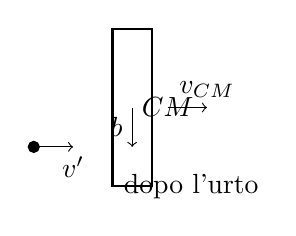
\begin{tikzpicture}
% sbarretta
\draw[thick] (2, -1) rectangle (2.5, 1);
\node at (2.7, 0) {$CM$};
\draw[->] (2.7, 0) -- (3.2, 0) node[above] {$v_{CM}$};
% proiettile
\filldraw (1, -0.5) circle (2pt);
\draw[->] (1, -0.5) -- (1.5, -0.5) node[below] {$v'$};
\draw[->] (2.25, 0) -- (2.25, -0.5) node[midway, left] {$b$};
\node at (3, -1) {dopo l'urto};
\end{tikzpicture}
\end{figure}

$$ 1 + \frac{M}{m} + \frac{12 b^2}{L^2} - \frac{2 v_0}{v_{CM}} = 0 \text{ affinché } \Delta E = 0 $$
$$ \Rightarrow v_{CM} = \frac{2 m v_0 L^2}{(M+m)L^2 + 12mb^2} \quad \Rightarrow v' = v_0 \left( 1 - \frac{2 M L^2}{(M+m)L^2 + 12mb^2} \right) $$
$$ \Rightarrow \omega = \frac{24 m b v_0}{(M+m)L^2 + 12mb^2} $$

\subsubsection*{Caso 3: Urto centrale $\bar{b} = 0$}
Si tratta come un punto materiale.
\paragraph*{3.1 (anelastico)}
$$ \Rightarrow \omega = 0 \quad \Rightarrow v' = \frac{m v_0}{m+M} \quad \Rightarrow v_{CM} = v' = \frac{m v_0}{m+M} $$
$$ \Rightarrow \Delta E = K_{rel} = \frac{-m M}{m+M} \cdot \frac{v_0^2}{2} = - \frac{1}{2} \mu v_0^2 $$

\paragraph*{3.2 (elastico)}
$$ \Rightarrow \omega = 0 \quad \Rightarrow v' = \left| \frac{m-M}{M+m} \right| v_0 \quad \Rightarrow v_{CM} = \frac{2 v_0 m}{m+M} $$

\subsection*{Esempio 2}
Urto di un proiettile $m$ con una sbarretta $M, L$ vincolata ad un perno liscio passante x un estremo. \textbf{trattazione generale}

\begin{figure}[H]
\raggedleft
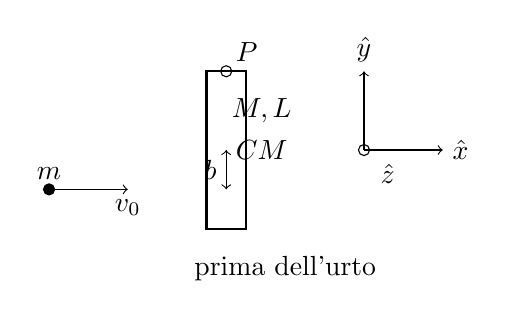
\begin{tikzpicture}
% perno P
\draw (2.25, 1) circle (2pt) node[above right] {$P$};
% sbarretta
\draw[thick] (2, -1) rectangle (2.5, 1);
\node at (2.7, 0) {$CM$};
\node at (2.7, 0.5) {$M, L$};
% proiettile
\filldraw (0, -0.5) circle (2pt) node[above] {$m$};
\draw[->] (0, -0.5) -- (1, -0.5) node[below] {$v_0$};
\draw[<->] (2.25, 0) -- (2.25, -0.5) node[midway, left] {$b$};
\node at (3, -1.5) {prima dell'urto};
% assi
\draw[->] (4, 0) -- (5, 0) node[right] {$\hat{x}$};
\draw[->] (4, 0) -- (4, 1) node[above] {$\hat{y}$};
\draw[->] (4, 0) circle (2pt);
\node at (4.3, -0.3) {$\hat{z}$};
\end{tikzpicture}
\end{figure}

- Forza impulsiva di $P \rightarrow$ SISTEMA NON ISOLATO: $\Delta \bar{P} \neq 0$
$$ \bar{P}_i = \bar{P}_{mi} + \bar{P}_{Mi} = m\bar{v}_0 + 0 \quad \bar{P}_f = \bar{P}_{mf} + \bar{P}_{Mf} = m\bar{v}' + M\bar{v}_{CM} $$
$$ \Rightarrow \Delta \bar{P} = m\bar{v}' + M\bar{v}_{CM} - m\bar{v}_0 = m(\bar{v}' - \bar{v}_0) + M \frac{L \omega}{2} \hat{x} $$
$\bar{v}_0 = v_0 \hat{x}, \bar{b} = -b \hat{y}$

- no momenti forze esterne su $P \rightarrow$ braccio nullo: $\bar{L}_O \text{ costante} = \bar{L}_P$
($O \equiv P$ (per il CM ad esempio non vale $\bar{L}_{CM} \text{ costante}$).
$$ \bar{L}_P^i = \left(\bar{b} + \frac{\bar{L}}{2}\right) \times \bar{p}_i = m\left(\bar{b} + \frac{\bar{L}}{2}\right) \times \bar{v}_0 = \bar{L}_P^f = \left(\bar{b} + \frac{\bar{L}}{2}\right) \times \bar{p}_f = m\left(\bar{b} + \frac{\bar{L}}{2}\right) \times \bar{v}' + \underbrace{I_P \bar{\omega}}_{= ML^2/3 \cdot \omega} $$
$$ \Rightarrow v' = v_0 - \frac{2}{3} \frac{M L^2 \omega}{m(L+2b)} $$
- rotazione intorno a P (no traslazione $\Rightarrow \bar{v}_{CM} = \bar{\omega} \cdot \bar{L}/2$)

- l'energia dipende dal tipo di urto
\begin{align*}
K_i &= K_{mi} = \frac{1}{2} m v_0^2 \\
K_f &= K_{mf} + K_{Mf} = \frac{1}{2} (m v'^2 + I_P \omega^2) \\
&= \frac{1}{2} \left( m v'^2 + \frac{1}{3} M L^2 \omega^2 \right)
\end{align*}

$$ \Rightarrow \Delta E = K_f - K_i = \frac{1}{3} M L^2 \omega^2 \left( \frac{1}{2} + \frac{2}{3} \frac{M L^2}{m(L+2b)^2} - \frac{2 v_0}{\omega(L+2b)} \right) $$

*
$$ \bar{v}_{CM} = \bar{\omega} \times \bar{r} = \omega \cdot r \cdot \sin(\theta_{\omega, r}) $$
